\documentclass[12pt]{article}

\usepackage[utf8]{inputenc}
\usepackage[russian]{babel}
\usepackage[normalem]{ulem}
\usepackage{amsmath, amssymb, titletoc, titlesec, tikz, pgfplots, csquotes, tabularx, fontspec, graphicx, caption, indentfirst}
\usepackage[top=2cm, bottom=2cm, left=2cm, right=1cm]{geometry}

\setmainfont{Times New Roman}
\linespread{1.25}

\begin{document}
\begin{center}
Министерство образования и науки Российской Федерации Федеральное государственное бюджетное образовательное учреждение высшего профессионального образования\\ \bigskip \textbf{\enquote{Московский государственный технический университет имени Н.Э. Баумана} \\ \smallskip (МГТУ им. Н. Э. Баумана)}
\end{center}
\noindent\rule{\textwidth}{1pt}
\smallskip\\
ФАКУЛЬТЕТ \enquote{Информатика и системы управления} \smallskip\\
КАФЕДРА \enquote{Теоретическая информатика и компьютерные технологии}\\
\bigskip\\
\begin{center}
\Large{\textbf{РАСЧЕТНО-ПОЯСНИТЕЛЬНАЯ ЗАПИСКА К КУРСОВОМУ ПРОЕКТУ НА ТЕМУ: \bigskip\bigskip\\
\textit{\enquote{Алгоритм глобального освещения для сцены с диффузными поверхностями}}}}
\end{center}
\vfill
\begin{tabularx}{\textwidth}{X c r}
Студент ИУ9-52 & $\underset{\text{(Подпись, дата)}}{\makebox[2.0in]{\hrulefill}}$ & А.А. Олохтонов\\
& & \\
Руководитель курсового проекта  & $\underset{\text{(Подпись, дата)}}{\makebox[2.0in]{\hrulefill}}$ & И.Э. Вишняков \bigskip\bigskip\\
\end{tabularx}
\begin{center}
Москва, 2017 г.
\end{center}
\thispagestyle{empty}

\newpage
\tableofcontents
\newpage

\section*{Введение}
\addcontentsline{toc}{section}{Введение}
Генерация реалистичных изображений --- направление компьютерной графики, ставящее своей целью преобразование описания произвольной сцены в изображение, минимально отличающееся от полученного при фотографировании реальной сцены (если таковая существует или может быть сконструирована). Для получения такого изображения необходимо произвести симуляцию процесса распространения света, и, с использованием полученных данных, расчитать для каждой выбранной единицы дискретизации (пикселя, вершины полигона и т.п.) значение энергетической яркости (англ: radiance).

В действительности самая полная на данный момент модель, описывающая поведение световых частиц --- кватновая --- слишком подробна для такой относительно простой цели, как генерация изображений. Упрощенный вариант квантовой модели, называемой \emph{волновой}, описывает процессы распространения света и его взаимодействия с объектами, сравнимыми с длиной световой волны (проявления такого взаимодействия можно наблюдать в таких эффектах как дифракция, интерференция и поляризация), с помощью уравнений Максвелла; но для целей компьютерной графики в большинстве случаев допустимо предположение, что все объекты много больше длины световой волны.

Добавив к описанному предположения о том, что свет распространяется в абсолютно прозрачной среде и преодолевает любую дистанцию мгновенно, можно получить т.н. модель \emph{геометрической оптики}, опирающуюся на понятие светового луча и подчиняющуюся всем знакомым законам отражения и преломления. Все описанные в данной курсовой работе алгоритмы используют именно такую модель, которая, не смотря на все упрощения, позволяет генерировать фотореалистичные изоражения.

Для генерации реалистичных изорбажений сцены, объекты которой обладают ничем не ограниченным наобром известных заранее отражающих свойств, существует множество алгоритмов, как основанных на классическом алгоритме трассировки лучей: трассировка путей (англ: path tracing), трассировка света (англ: light tracing), так и принципиально иных, таких как метод фотонных карт (англ: photon mapping), кэш освещенности (англ: irradiance caching) и др. Однако в случае, если все объекты сцены обладают диффузными поверхностями (распространают отраженный свет по закону Ламберта), для расчета освещенности сцены возможно использовать иной алгоритм, называемый \emph{методом излучаемости (англ: radiosity)}. В установленных ограничениях этот метод позволяет получить физически корректные значения освещенности, коль скоро точно заданы параметры сцены. 

Целью данной курсовой работы является подробное изучение и реализация метода излучаемости, а так же обнаружение, анализ и последующее решение проблем, свойственных данному алгоритму. В работу также входит подробное тестрирование полученной реализации, включающее в себя оценку производительности и описание созданных отладочных инструментов. В ходе выполнения курсовой работы решаются следующие задачи: обзор алгоритмов глобольного освещения, определние специфики сцен с диффузными поверхностями, разработка алгоритма, основанного на методе излучаемости, и анализ возможных модификаций, разработка структуры приложения, проработка и описание деталей реализации и тестирования.
\newpage\section{Алгоритмы глобального освещения}
Алгоритмами глобального освещения называют семейство алгоритмов, направленных на реалистичую симуляцию процессов отражения, рассеивания, поглащения и преломления света, т.е. на расчет распределения света в рамках модели геометрической оптики. Но что скрывается под фразой ``реалистичная симуляция'' и что именно расчитывается в алгоритмах глобального освещения? Ответ на вторую часть этого вопроса напрямую зависит от выбранного алгоритма, однако проблема ``симуляции'' световых явлений была сформулирована математически Д. Кажия в 1986 г. \cite{Kaj86} в виде интегрального уравнения, называемого ``уравнением рендеринга'', современная форма которого имеет следующий вид:
\begin{equation}
L_0(x, \omega_o, \lambda, t) = L_e(x, \omega_o, \lambda, t) + \int_\Omega f_r(x, \omega_i, \omega_0, \lambda, t) L_i(x, \omega_i, \lambda, t) (\omega_i \cdot n) d\omega_i, \label{eq:kaj}
\end{equation}
где $L_0(x, \omega_o, \lambda, t)$ --- спектральная энергетическая яркость в точке $x$ на длине в направлении $\omega_0$ на длине волны $\lambda$ в момент времени $t$, $L_e(x, \omega_o, \lambda, t)$ --- излучаемая энергетическая яркость (не равна нулю только для точек, излучающих свет), $\int_\Omega d\omega_i$ --- интеграл по единичному полушарию $\Omega$ вокруг нормали $n$ к поверхности в точке $x$, $f_r(x, \omega_i, \omega_0, \lambda, t)$ --- двулучевая функция отражательной способности (англ: bidirectional reflectance distribution function, BRDF) в точке $x$, параметризованная направлением к позиции наблюдателя $\omega_0$ и направлением к источнику света $\omega_i$. $L_i(x, \omega_i, \lambda, t)$ описывает спектральную энергетическую яркость, направленную в точку $x$ с направления $\omega_i$, а скалярное произведение $(\omega_i \cdot n)$ --- ослабление освещенности, вызванное увеличенным углом падения.

Так как подынтрегральноая величина $L_i$ сама в свою очередь выражается аналогично, для получения решения этого уравнения даже в одной точке необходимо вычислить бесконечномерный интеграл, что не представляется возможным. По этой причине любое ``решение'' уравнения рендеринга представляет собой лишь приближение, получаемое численными методами. Из выбора такого метода и проистекают различные алгоритмы глобального освещения.
\subsection{Трассировка лучей}
При описании алгоритмов глобального освещения нельзя не упомянуть алгоритм трассировки лучей, истоком которого принято считать работу Т. Виттеда \cite{Witt80}, представленную в 1980 г. Однако описанная модель была неполной, и не решала уравнение рендеринга (которое на тот момент еще не было сформулировано), а включала в себя только обнаружение видимых граней и отображение идеальных отражателей и преломителей. Позже алгоритм был модифицирован (в том числе самим Д. Кажия в \cite{Kaj86}) для решения полного уравнения рендеринга и, как следствие, с его помощью стало возможно получать изображения световых явлений любой степени сложности в рамках геометрической модели оптики.

Одним из самых популярных современных вариантов алгоритма трассировки лучей является так назыаемый алгоритм ``трассировки путей'' (англ: path tracing), в ходе которого для каждого пикселя вычисляется приближенное интеграла
\begin{equation}
L_{\text{пиксель}} = \int_{\text{экран}} L(x \rightarrow e) h(p) dp,\label{eq:pt}
\end{equation}
где p пробегает все точки экрана внутри данного пикселя, а x --- точка сцены, которую ``видно'' при взгляде с позиции e в направлении точки p. Чаще всего функция h(p) представляет собой такую фильтрующую функцию, что итоговая энергетическая яркость пикселя равняется среднему арифмитическому всех вычисленных значений внутри данного пикселя, однако возможны и более сложные модели, в которых роль виртуальной камеры играет уже не стеноп (англ: pinhole), а более реалистичная модель с виртуальной линзой \cite{Kolb95}.

Подстановка на место $L(x \rightarrow e)$ из уравнения \eqref{eq:pt} правой части уравнения \eqref{eq:kaj} дает интеграл, решение которого можно непосредственно (после тонирования) использовать для отображения получившейся картинки.

Для решения описанного интеграла используют метод численного интрегирования Монте-Карло: расчет приближенного значения интеграла производится с помощью набора случайных точек из области интегрирования, значения в которых взвешенно усредняются. Ключевым в данном случае является выбор оценочной функции, от которого зависит как то, будут ли получаемые решения сходиться к верному при увеличении выборки, так и скорость такой сходимости. Простейшим примером использования численного интегрирования Монте-Карло для решения уравнения \eqref{eq:pt} является равномерная выборка, при которой точки выбираются из области интегрирования с вероятностью $p = \dfrac{1}{M}$, где $M$ --- мера области выборки (таковой может являться площадь пикселя или рассматриваемый телесный угол), и сумма полученных значений делится на $N$. В таком случае оценочная сумма для интеграла из уравнения \eqref{eq:kaj} принимает вид
\begin{equation}
\frac{1}{N} \sum_{i = 1}^{N} \frac{L(x \leftarrow \omega_i) f_r(x, \omega, \omega_i) \cos(\omega_i, N_x)}{pdf(\omega_i)}, \label{eq:mc-kaj}
\end{equation}
где $\omega_i$ --- направление из полушария вокруг нормали $N_x$ к поверхности сцены в точке $x$, $f_r(x, \omega, \omega_i)$ --- ДФОС в точке $x$ при взгляде по направлению, противоположному $\omega$, $\cos(\omega_i, N_x)$ --- фактор затухания, а $pdf(\omega_i)$ --- вероятность выбора направления $\omega_i$ (т.н. плотность вероятности, англ: probability density function), которая зависит от выбранной параметризации полушария. Значения ДФОС, плотности и затухания извлекаются непосредственно из описания сцены, а значение $L(x \leftarrow \omega_i)$ вычисляется по аналогичной формуле, где на месте $\omega$ будет стоять уже $\omega_i$. На практике такие расчеты чаще всего реализуются с помощью рекурсии или итерации, условием остановки которых является превышение максимального количество итераций или глубины рекурсии, либо попадание в точку, имеющую ненулевую собственную излучаемость $L_e$ (т.е. являющуюся источником света).

В описанном виде алгоритм трассировки путей крайне неэффективен и для большинства сцен генерирует за любое разумное время очень ``шумное'' изображение, так как большое количество путей так и не попадает в источник света. При увеличении выборки получаемые изображения рано или поздно сойдутся к верному решению, однако во многих случаях необходимое для этого количество времени представляется непрактичным: к примеру, отрисовка сцены, освещаемой удаленным и небольшим, но очень ярким источником света может занять недели или даже месяцы. За разумное же время без дополнительных модификаций трассировка путей генерирует следующие изображения \cite{karlIMP, karlBDPT}:
\begin{figure}[h]
\centering
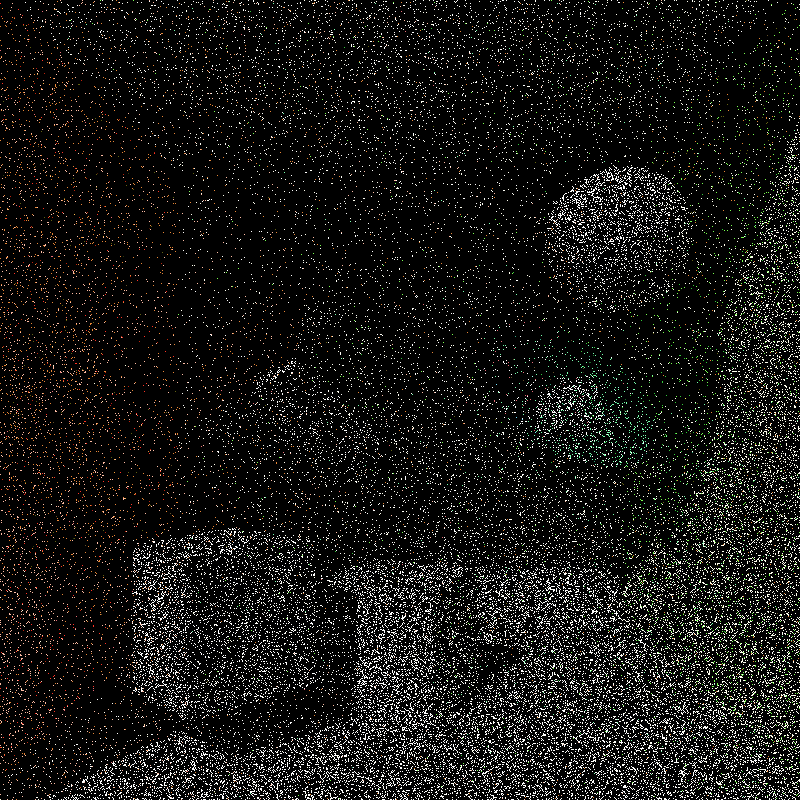
\includegraphics[scale=0.3]{indirect5120.png}
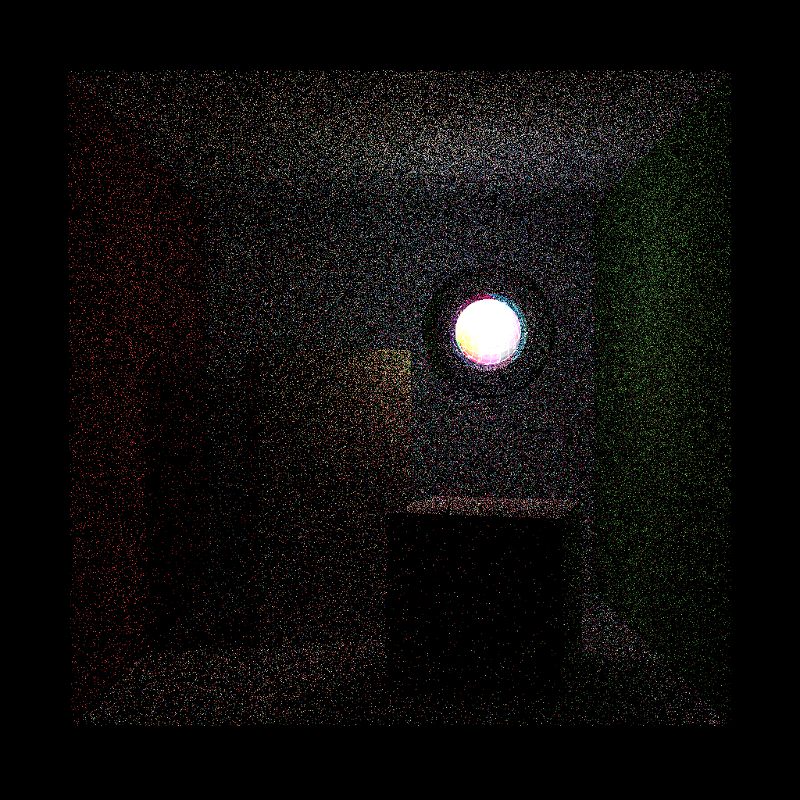
\includegraphics[scale=0.3]{spherelight_16.png}
\caption*{Рисунок 1 --- Неэффективно рассчитанные трассировкой путей сцены}
\end{figure}

Производительность алгоритма трассировки путей может быть многократно увеличена при помощи использования техник уменьшения дисперсии, програмных оптимизаций и различных эвристик, некоторые из которых затронуты в последующих главах данной курсовой работы.

Из главного преимущества алгоритма трассировки лучей --- универсальности --- следует и его главный недостаток: решение уравнения \eqref{eq:pt} подразумевает фиксацию позиции наблюдателя и, следовательно, представляет собой неподвижное изображение. Теоретически, алгоритм возможно адаптировать для расчета значений в вершинах сцены, заданной полигональной сеткой, однако практика показывает, что такой подход крайне неэффективен.

Для сцен с диффузными поверхностями, т.е. таких, где все ДФОС во всех точках имеет вид $f_r(x) = \dfrac{\rho}{\pi}$, алгоритм трассировки путей также работает крайне неэффективно по той причине, что для расчета излучаемости в таких точках требуется очень большая выборка, которая, из-за рекурсивной природы алгоритма, приводит к запредельным временам расчета для большинства нетривиальных сцен.
\subsection{Метод излучательности}
Помимо алгоритмов, основанных на трассировке лучей, существуют и другие, решающие схожую, но не такую же задачу: расчет освещенности сцены, где каждая точка (поверхность) является рассеивающим отражателем (ДФОС во всех точках равна $\dfrac{\rho}{\pi}$). Для такой сцены уравнение \eqref{eq:kaj} принимает вид
\begin{equation}
L(x) = L_e(x) + \int_{\Omega} f_r(x) L(x \leftarrow \omega_i) \cos(\omega_i, N_x) d \omega_i, \label{eq:diff-kaj}
\end{equation}
то есть не зависит от позиции наблюдателя. В указанных ограничениях возможно получить решение, которое не привязано к одному направленю взгляда и может (по окончанию расчетов) быть использовано для составления интерактивной трехмерной модели.

Одним из таких алгоритмов является \emph{метод излучаемости}, основанный на алгоритме расчета теплопередачи и впервые адпатированный для генерации реалистичных изображений в 1984 г. \cite{Gor84}. Основная идея алгоритма заключается в том, что поверхности сцены разбиваются на участки, излучательность на которых полагается константной, и распределение энергии расчитывается между этими участками. Для каждого такого участка входными данными является его собственная излучаемость $B_i^e$ (описывающая его яркость) и отражательная способность $\rho_i$ (в диапозоне от нуля до единицы). За участки часто принимаются полигоны, описывающие сцену, если такая информация доступна.

Следующим шагом решается система линейных уравнений, связывающая излучаемость всех участков сцены. Итогом решения такой системы являются значения $B_i$ для каждого участка, которые затем переводятся в яркость процессом тонирования и могут быть отображены на экране с помощью растеризации. Так как вычисленные значения не зависят от позиции наблюдателя, использование графических ускорителей позволяет визуализировать ``освещенную'' сцену в реальном времени с произвольной позиции.
\begin{figure}[h]
\centering
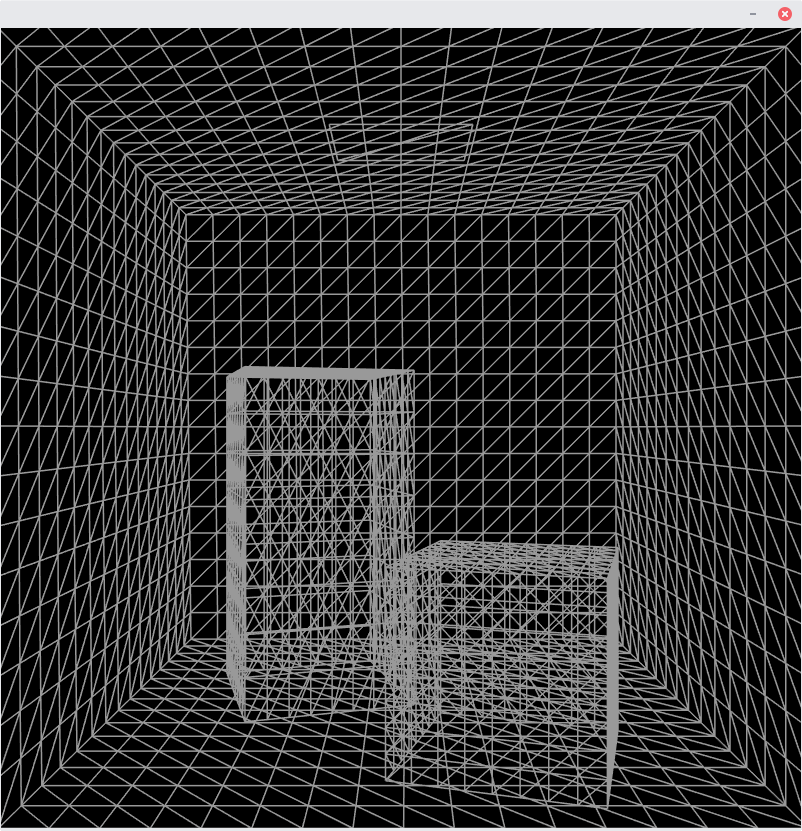
\includegraphics[scale=0.3]{rad_input.png}
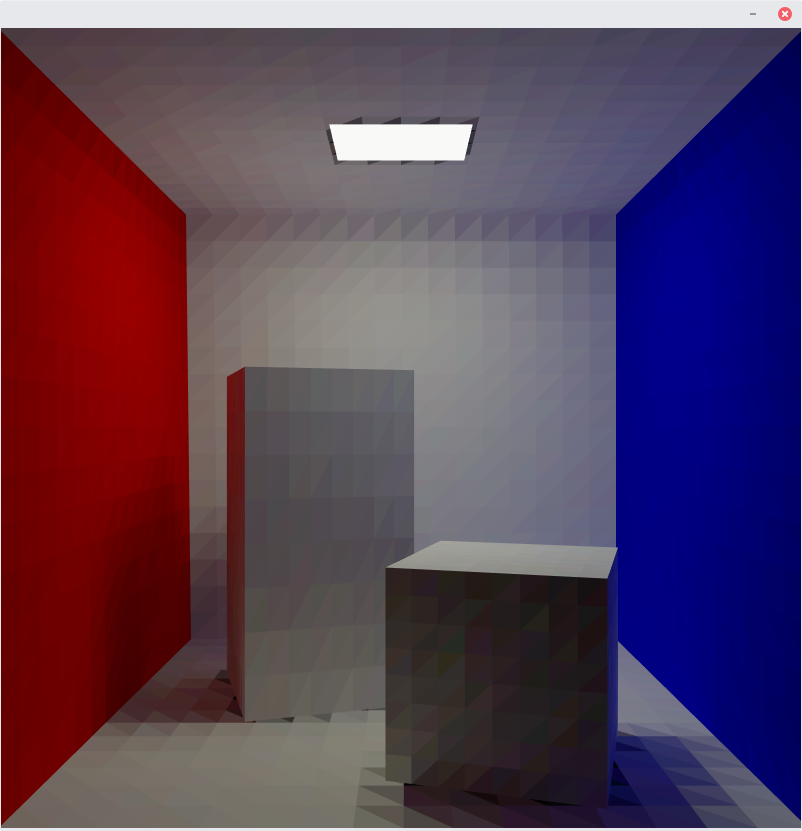
\includegraphics[scale=0.3]{rad_output.png}
\caption*{Рисунок 2 --- Метод излучательности}
\end{figure}

Классический метод излучательности представляет собой частный случай более общего численного метода --- \emph{метода конечных элементов}, широко использующегося в решении задачач гидродинамики, электродинамики и теплообмена. Вкратце, математическое основание метода заключается в следующем: из уравнения \eqref{eq:diff-kaj} выводится СЛАУ путем переформулировки интеграла по полушарию на интеграл по всем поверхностям сцены:
\begin{equation}
L(x) = L_e(x) + \rho(x) \int_S K(x, y) L(y) d A_y, \label{eq:kaj-surf}
\end{equation}
ядром интегрирования которой служит функция $K(x,y)$, равная произведению $G(x,y) V(x,y)$, где 
\begin{equation}
G(x,y) = \frac{\cos(\theta_{xy}, N_x) \cos(-\theta_{xy}, N_y)}{\pi r_{xy}^2}\label{eq:geom}
\end{equation}
описывает взаимную ориентацию поверхностей в пространстве, а $V(x,y)$ равняется 1, если точки $x$ и $y$ взаимно видимы, и нулю в противном случае. Затем, полученное равенство используется для выражения средней излучаемости $B_i$ произвольной поверхности, после чего излучаемость полагается константой на каждом выделенном участке, и интеграл можно переписать как сумму \cite{Coh93}:
\begin{equation}
\begin{split}
&B_i = B_{ei} + \rho_i \sum_j F_{ij} B_j\\
&F_{ij} = \frac{1}{A_i} \int_{S_i} \int_{S_j} K(x,y) dA_y dA_x, \label{eq:rad}
\end{split}
\end{equation}
систему которых (для всех $i$) называют \emph{системой уравнений метода излучательности}. Коэффициенты $F_{ij}$ обычно называют \emph{форм-факторами}: их вычисление и хранение служат причиной большинства проблем, связанных с реализацией метода. Как только коэффициенты системы расчитаны, остается применить один из методов решения СЛАУ для получения искомых величин.

Следующая глава данной курсовой работы посвящена описанию и анализу классического метода излучательности, проблем, сопровождающих реализацию оного, и представлению различных модификаций, решающих эти проблемы.
\newpage\section{Разработка алгоритма}
\subsection{Стандартный метод излучательности}
Концептуально, классический метод излучательности состоит из следующих шагов:
\begin{enumerate}
\item[1)] дискретизация входных данных на участки, излучаемость на которых полагается константной (для данной длины волны);
\item[2)] расчет форм-факторов $F_{ij}$ для всех пар $(i, j)$ участков получившейся сцены;
\item[3)] численное решение системы уравнений \eqref{eq:rad};
\item[4)] отображение решения (включает в себя как процесс тонирования, так и преобразование спектральных данных в необходимое требуемое пространство).
\end{enumerate}

Каждый из приведенных шагов может быть реализован с использованием различных методов, выбор которых определяет не только время работы алгоритма, но и количество необходимых для его работы ресурсов: так, форм-факторы могут быть рассчитаны заранее и сохранены в памяти для дальнейшего использования, а могут рассчитываться заново по необходимости.

Последний, четвертый, шаг алгоритма представляет меньше трудностей нежели остальные: физический смысл происходящего прост и понятен, а реализация сводится к выбору оператора тонирования, подробно описанному в главе 3.5. Первым же трем шагам сопутствуют трудности, преодоление некоторых из которых как минимум нетривиально. Далее будут описаны проблемы, сопровождающие реализацию метода излучательности в том виде, в котором он представлен в начале настоящей главы.

На первый взгляд это может показаться неочевидным, но даже реализация первого этапа алгоритма вызывает трудности. Для достижения реалистичного результата участки, на которые разбивается сцена, должны быть достаточно небольшими, чтобы передавать все детали освещения (например, на границе резких теней), однако излишнее измельчение сцены приведет к неадекватным временным затратам и требованиям к доступной памяти. В идеале процесс дискретизации сцены должен гарантировать с заданной точностью, что на каждом полученном участке излучаемость будет постоянной.

Больше всего проблем, бесспорно, связано со вторым этапом алгоритма: расчетом и хранением форм-факторов. Во-первых, форм-фактор представляет собой двойной интеграл по поверхности, т.е. для получения искомого значения необходимо решить дифференциальное уравнение четвертой степени, которое  ``даже самого терпиливого преисполнит отвращения'' \cite{Sch93}. Более того, аналитически решение возможно получить только в частом случае взаимно видимых поверхностей, практически не встречающемся в задаче генерации реалистичных изображений. В остальных же случаях интеграл вычислим лишь численными методами, так или иначе включающими в себя многократную проверку взаимной видимости двух произвольных точек сцены. Не облегчает ситуации и тот факт, что подынтегральная функция может иметь разрывы разных степеней, и $r_{xy}^2$ в знаменателе может стремиться к нулю для двух смежных участков. Однако самой серьезной проблемой для любых нетривиальных сцен всегда является количество вычисляемых форм-факторов: в более сложных моделях количество полигонов может исчисляться миллионами, а количество вычисляемых форм-факторов, следовательно, --- триллионами, что далеко выходит за рамки возможностей современных ПК. Вместе с тем, как замечено ранее, недостаточная гранулярность разбиения приводит потерям деталей и нарушению реализма:
\begin{figure}[h]
\centering
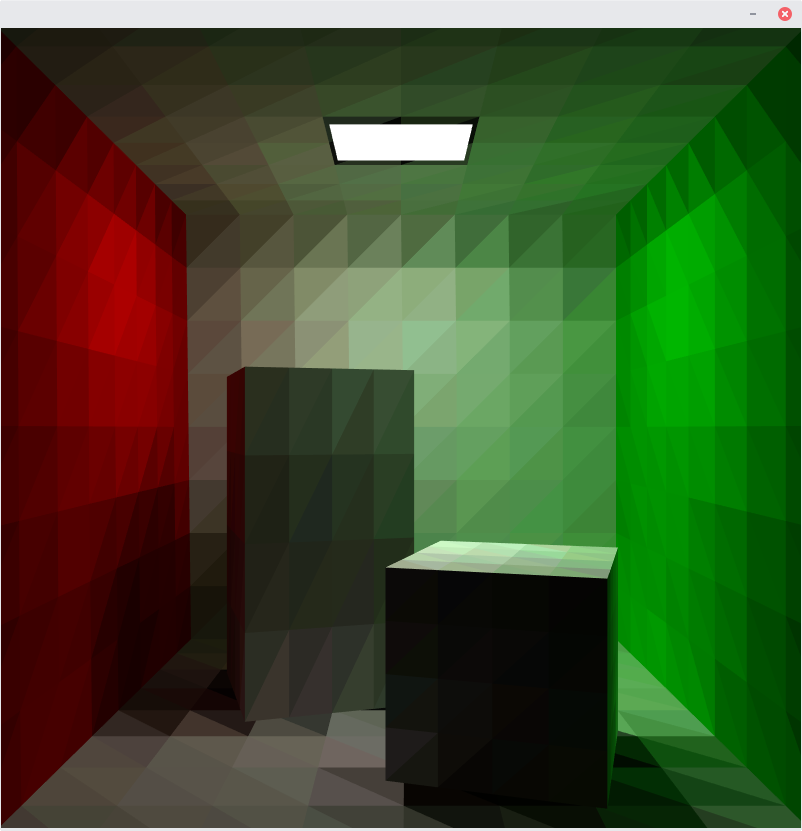
\includegraphics[scale=0.3]{rad_bad1.png}
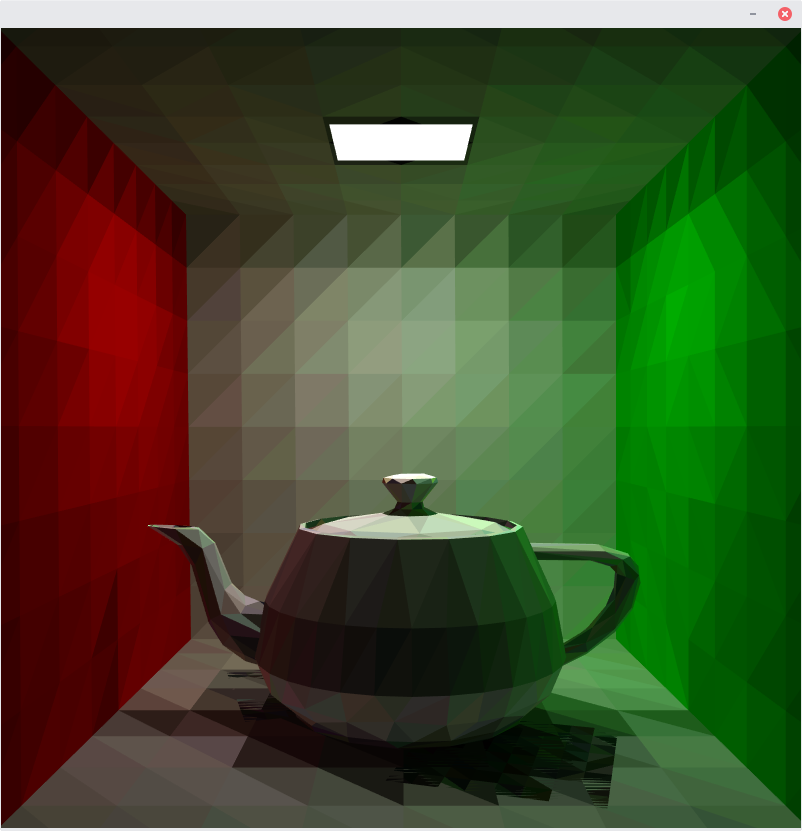
\includegraphics[scale=0.3]{rad_bad2.png}
\caption*{Рисунок 3 --- Артефакты при недостаточном разбиении}
\end{figure}

Решение системы уравнений излучательности \eqref{eq:rad} сложной сцены детерминистскими методами также нецелесообразно из-за необходимости хранения форм-факторов.
\subsection{Итеративный подход}
Заметим, что матрица коэффициентов системы уравнений излучательности обладает свойством диагонального преобладания \cite{Pet06}, что позволяет использовать итеративный метод Якоби для получения решения с любой требуемой точностью. Использование итеративного подхода допускает расчет только одной строки форм-факторов в любой момент времени, так как в процессе итерации уточненные значения рассчитываются для каждого участка независимо. Таким образом, проблема хранения квадратичного числа форм-факторов решается в корню. Более того, каждая такая итерация отвечает одному отражению всех световых лучей сцены, что интуитивно понятнее, чем расчет ``всех'' отражений для каждого луча по очереди, и позволяет тривиально организовать процесс предпросмотра получаемого решения.

Более конкретно, итеративный процесс Якоби применим к решению СЛАУ излучательности следующим образом: начальными значениями излучаемости для каждого участка полагается их собственная излучаемость (положительная для источников света и ноль для остальных). Далее, значения последовательно уточняются с использованием приближений, полученных на предыдущей итерации. Приминительно к системе \eqref{eq:rad} использование итеративного метода Якоби дает для каждого участка $i$ следующее выражение:
\begin{equation}
\begin{split}
B_i^{(0)} &= B_{ei}\\
B_i^{(k + 1)} &= B_{ei} + \rho_i \sum_j F_{ij} B_j^{(k)}.\label{eq:iter}
\end{split}
\end{equation}
С использованием метода полукуба \cite{Coh85}, позволяющим получить сразу всю строку форм-факторов для данного участка, становится возможной генерация следующего изображения \cite{Coh85}:
\begin{figure}[h]
\centering
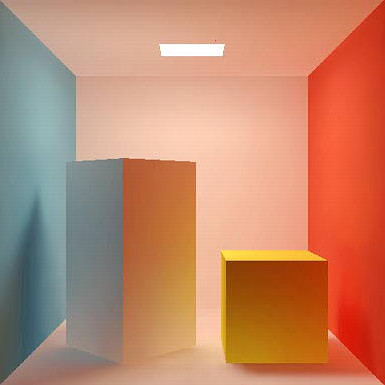
\includegraphics[scale=0.647]{cohen.jpg}
\caption*{Рисунок 4 --- Решение СЛАУ излучательности итеративным методом Якоби}
\end{figure}

Применение итераций Якоби для решения системы уравнений излучательности позволяет не только избавиться от необходимости хранения всех пар форм-факторов в явном виде, но и предоставляет интуитивно понятный процесс получения последовательных приближений. Так, для расчета локальной модели освещения достаточно остановить итеративный процесс после первого же приближения (см. рис. 5).

Однако, хоть проблема хранения и решается описанным методом, сохраняет свою актуальность вопрос вычисления форм-факторов: для получения одного приближения необходимо произвести квадратично зависимое от $N$ число вычислений: $N \cdot (N - 1)~/~2$ двойных интегралов по поверхностям. Сверх того, отказ от хранения форм-факторов приводит к тому, что на кажой итерации значения рассчитываются заново! Из этого следует, в том числе, что при недостаточно точно вычисляемых значениях форм-факторов, используемые итерации могут вообще не дать годного к использованию решения за адекватное время.

В следующей главе представлен т.н. \emph{метод локальных линий}, в котором форм-факторы рассматриваются как вероятности, и потому могут быть приближены с использованием статистических методов и, что самое главное, вычисляться неявно, в следствие чего проблемы хранения и повторного вычисления форм-факторов попросту исчезают. 


\begin{figure}[h]
\centering
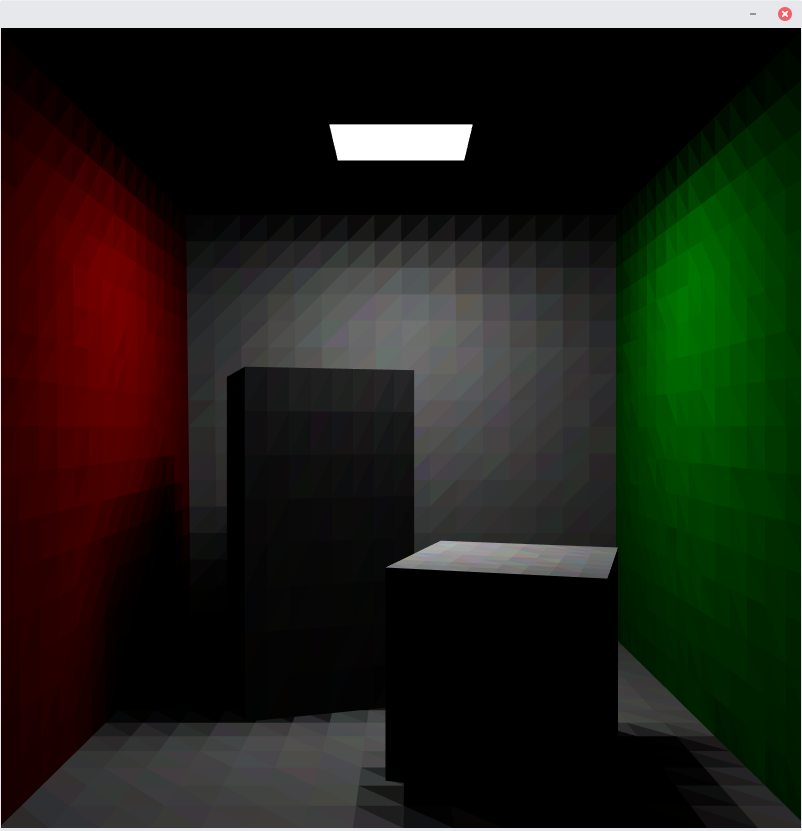
\includegraphics[scale=0.3]{direct_only.png}
\caption*{Рисунок 5 --- Результат работы одной итерации алгоритма}
\end{figure}

\subsection{Метод локальных линий}
Рассмотрим формулу для форм-факторов из уравнения \eqref{eq:rad}: значение подынтегральной функции, а значит и самого интеграла, всегда принимает неотрицательные значения. Взглянем теперь на сумму всех форм-факторов $F_{ij}$ для фиксированного участка $i$:
\begin{equation}
\begin{split}
\sum_j F_{ij} &= \frac{1}{A_i} \int_{S_i} \sum_j \int_{S_j} K(x,y) dA_y dA_x = \\
&= \frac{1}{A_i} \int_S K(x,y) dA_y dA_x.
\label{eq:ff-sum}
\end{split}
\end{equation}
Переформулировав интеграл обратно в термины направлений, получим
\begin{equation}
\begin{split}
\sum_j F_{ij} &= \frac{1}{A_i} \int_{S_i} \frac{1}{\pi} \int_{\Omega_x} \cos(\theta_{xy}, N_x) d\theta_{xy} dA_x\\
&= \frac{1}{A_i} \int_{S_i} \frac{\pi}{\pi} dA_x= 1.
\label{eq:ff-sum2}
\end{split}
\end{equation}
Таким образом, сумма всех форм-факторов для данного участка равняется единице (в случае незамкнутой сцены сумма может принимать меньшие значения). Наконец заметим, что простая перестановка порядка интегралов позволяет убедиться, что для любых $i$, $j$
\begin{equation}
A_i F_{ij} = A_j F_{ji}.\label{eq:ff-rep}
\end{equation}
Перечисленный набор свойств позволяет рассматривать форм-факторы $F_{ij}$ как набор \emph{вероятностей}. Вспомним теперь, что (за вычетом собственной излучаемости) форм-фактор $F_{ij}$ описывает \emph{долю} излучаемости участка $i$, происходящюю от участка $j$. Учитывая, что энергия $P_i$ и излучаемость $B_i$ данного участка различаются лишь зависимостью от площади: $P_i = A_i B_i$, систему уравнений излучательности можно переформулировать с использованием энергии:
\begin{equation}
P_i = P_{ei} + \sum_j P_j F_{ji} \rho_i, \label{eq:rad-pow}
\end{equation}
где $F_{ji}$ обозначает часть энергии участка $i$ (за вычетом излучаемой), отвечающей участку $j$, или, что то же самое, $F_{ij}$ обозначает часть энергии участка $i$ (за вычетом излучаемой), попадающей на участок $j$. Такая формулировка позволяет получить приблизительное значение форм-факторов $F_{ij}$ для участка $i$ при помощи простейшей симуляции, выпустив $N_i$ лучей из случайных точек участка и распределенных согласно закону косинусов в полушаре вокруг нормали. Тогда отношение $N_j / N_i$ попавших в участок $j$ лучей к общему их числу будет приблизительно равно форм-фактору $F_{ij}$ \cite{Shir90}.
\begin{figure}[h]
\centering
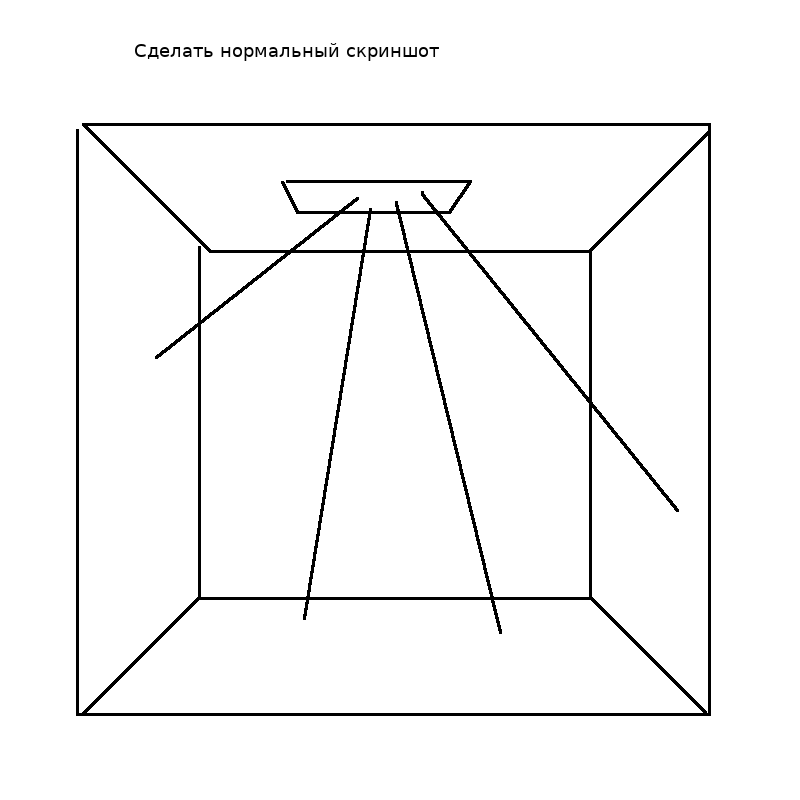
\includegraphics[scale=0.3]{local_lines.png}
\caption*{Рисунок 6 --- Расчет форм-факторов с использованием локальных линий}
\end{figure}

\begin{center}= = = здесь начинается черновой текст = = =\end{center}
Описанный процесс ценен в основном за идею, и не должен использоваться непосредственно, потому что форм-факторы до сих пор нужно считать и хранить. Самое главное, что мы получили другую формулировку пробелмы, которая позволяет использовать принципиально другие подходы к решению. Так, следующая глава посвящена использованию метода Монте-Карло для приближения суммы $\sum_j N_j$.

\subsection{Стохастический алгоритм}
Так вот, используем метод Монте-Карло для получения приблизительного значения искомой суммы. Это значение можно получить, если случайно выбирать члены суммы согласно некоторой вероятности, а затем усреднить все выбранные члены деленные на обратную вероятность их выбора. Более того, умный выбор переменных позволяет не хранить форм-факторы (мы так этого ждали!!). Итак, алгоритм. У нас есть есть итерации Якоби. У насть есть формулировка СЛАУ излучательнотси для ``невыстреленной'' энергии (ввести формулировку). В итерациях сумма для невыстреленной энергии $\Delta P_j^{(k+1)}$, которую мы и будем прикидывать. Для этого:
\begin{enumerate}
\item[1)] выбрать стрелающий участкок с вероятностью, равной доле невыстреленной энергии данного участка
\item[2)] выбрать второй участкой, просто затрейсив локальную линию. вероятность попадания в этот участой будет $F_ij$.
\end{enumerate}

Получается, что достаточно умно составить алгоритм, и тогда всё сократится. Анализ говорит (ссылка), что нужно трейсить линейное количество лучей до сходимости. При использовании структуры мы получаем логарифм для трейса каждого луча. Итого лог-линия, которая ГОРАЗДО лучше оригинального квадрата. Сверх того, отсутствие необходимости хранить форм-факторы позволяет рисовать по истине громадные сцены, которые невозможно было бы отобразить с использованием обычного алгоритма. 
\begin{figure}[h]
\centering
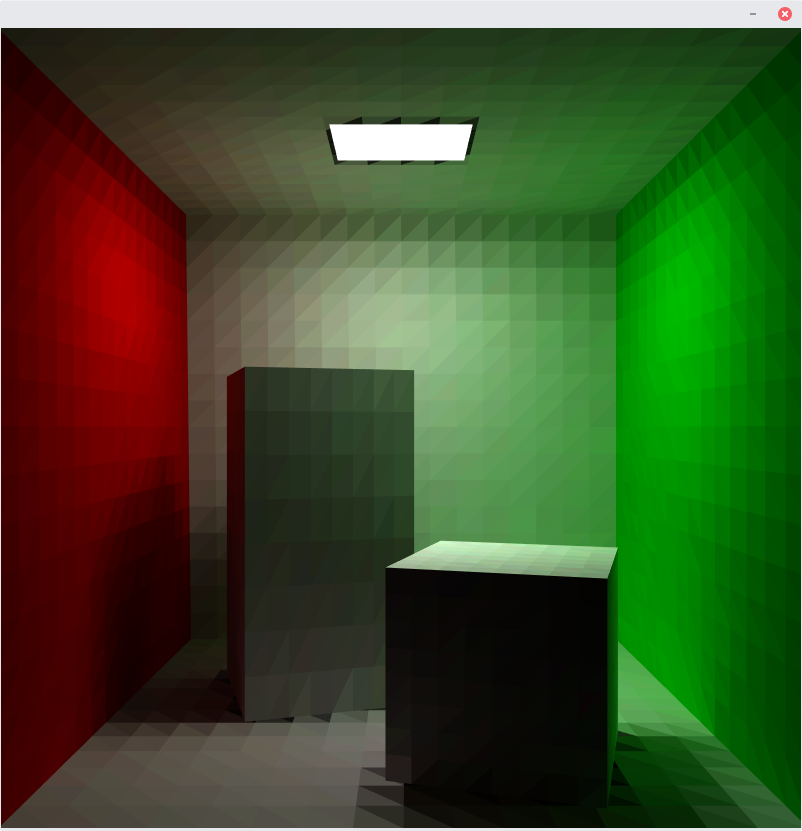
\includegraphics[scale=0.3]{rad_stoch.png}
\caption*{Рисунок 7 --- Результат работы стохастического алгоритма}
\end{figure}

Работает, довольно хорошо. Но что можно еще улучшить? Так как это Монте-Карло, то можно использовать различные техники снижения дисперсии, такие как: имп. семплинг, лоу диср. стратифайд, реджекшион, и т.д.. Некоторые из них описаны далее.
\subsection{Модификации и ускорения}
Как выбрать полигон - прямо конкретно про энергнию. Как считать число лучей, которые из него стрелять. Как считать количество лучей в сумме всего; как рендерить цвет; как смотреть промежуточный результат; как ускорить трейсинг (бвх). Получившийся алгоритм: \emph{псевдокод} + ссылка на \cite{Pet06}.
\newpage\section{Реализация}
% Писать на C++, рисовать через OpenGL. Линукс, glfw, glew. 
\subsection{Общая структура приложения}
% src/ includes/ models/  в main у нас всякие подгрузки, настройки (constants, чтобы не перекомпилить)
\subsection{Загрузка полигональной модели}
% tinyobj loader, patch = 3 vertices, emit, color, normal, area
\subsection{Построение BVH-дерева}
% краткое описание bvh, где лист, где не лист, простое деление пополам (std::partition), все только переставляет в массиве указателей, листинги + как потом пересекать bvh
\subsection{Расчет излучательности}
% для каждой длины волны, пока энергия в сумме не закончится, считаем количество лучей, стреляем лучами (описание функции sample_hemi), пересекаекм bvh, увеличиваем. по окончанию заполняем данные для oGL цветами (излучательностью)
\subsection{Тонирование}
% зачем это надо, фотки без тонирования, оператор Реинхарда, результаты
\subsection{Отображение результатов}
% функция glify, отрисовка в oGL, класс шейдера, класс камеры
\newpage\section{Тестирование}
\subsection{Оценка производительности}
% сравнить только ассимпотически с дефолтом, замерить bvh, быстрый рендер в не очень хорошем качестве
\subsection{Оценка результатов}
% как утекает цвет, мягкие тени, цветные тени. рендер в очень хорошем качестве, показать на минусы (нет адаптив сабдив, но это не входило в планы)
\subsection{Отладка}
% отдельные поток для расчетов, чтобы смотреть mesh. граф. отладка для лучей, отладочная печать
\newpage\section*{Заключение}
\addcontentsline{toc}{section}{Заключение}

\newpage
\begin{thebibliography}{9} % Источники
\addcontentsline{toc}{section}{Список литературы}
\bibitem{Kaj86} 
Kajiya J.
\textit{The Rendering Equation.} / 
J. Kajiya //
Computer Graphics (SIGGRAPH ’86 Proceedings) --- Dallas, 1986 --- С. 143-150.

\bibitem{Witt80} 
Whitted T.
\textit{An Improved Illumination Model for Shaded Display.} / 
T. Whitted //
Communications of the ACM --- 1980 --- С. 343–349.

\bibitem{Kolb95}
Kolb C.
\textit{A Realistic Camera Model for Computer Graphics.} /
C. Kolb, D. Mitchell, P. Hanrahan //
Computer Graphics (SIGGRAPH ’95 Proceedings) --- Los Angeles, 1995 --- С. 317-324.

\bibitem{karlIMP}
Yining K.
\textit{Importance Sampled Direct Lighting.} / 
Yining K. //
Code and Visuals --- 2013 --- Режим доступа: http://blog.yiningkarlli.com/2013/04/importance-sampled-direct-lighting.html (дата обращения 11.01.2018)

\bibitem{karlBDPT}
Yining K.
\textit{Bidirectional Pathtracing Integrator.} / 
Yining K. //
Code and Visuals --- 2015 --- Режим доступа: http://blog.yiningkarlli.com/2015/02/bidirectional-pathtracing-integrator.html (дата обращения 11.01.2018)

\bibitem{Gor84}
Goral C.
\textit{Modeling the Interaction of Light Between Diffuse Surfaces.} /
C. Goral, K. Torrance, D. Greenberg, B. Battaile //
Computer Graphics (SIGGRAPH ’84 Proceedings) --- Minneapolis, 1984 --- С. 213-222.

\bibitem{Coh93}
Cohen M.
\textit{Radiosity and Realistic Image Synthesis} /Shir90
M. Cohen, J. Wallace
--- Boston: Academic Press Professional, 1993 --- 381 с.

\bibitem{Sch93}
Schr{\"o}der P.
\textit{A closed form expression for the form factor between two polygons} /
P. Schr{\"o}der, P. Hanrahan //
Tech. Rep. CS-404-93 --- Department of Computer Science, Princeton University, 1993.

\bibitem{Pet06}
Peters A.
\textit{Advanced Global Illumination, Second Edition} /
A. Peters, P. Dutre, K. Bala
--- Wellesley, Massachusetts: A K Peters Ltd/CRC Press, 2006 --- 384 c.

\bibitem{Coh85}
Cohen M.
\textit{The Hemi-Cube, A Radiosity Solution for Complex Environments} /
M. Cohen, D. Greenberg //
Computer Graphics (SIGGRAPH ’85 Proceedings) --- San Francisco, 1985 --- С. 31-40.

\bibitem{Shir90}
P. Shirley
\textit{A Ray Tracing Method for Illumination Calculation in Diffuse–Specular Scenes.} /
P.Shirley //
Graphics Interface '90 --- 1990 --- С. 205–212.
1990.


\end{thebibliography}
\newpage
Термины:

\begin{itemize}
\item[] 'radiosity' --- метод излучательности
\item[] 'radiance' --- энергетическая яркость
\item[] 'importance sampling' --- выборка по значимости
\item[] 'tone mapping' --- тонирование (???)
\item[] 'sample' --- выборка
\end{itemize}
\end{document}